\section{Prototipação de Baixa Fidelidade}

\subsection{Cenário Textual}

Ao não se sentir bem, um usuário busca na internet por um sistema de diagnóstico online.
Esse usuário sabe que simplesmente buscar por sintomas de maneira isolada não leva a dados concretos.

Nesse contexto, este usuário encontra o sistema HealthWeb, onde, após concordar com os termos de uso, preenche alguns dados simples, como sexo, idade e peso, então segue para um questionário com perguntas do tipo sim e não a respeito de sintomas que tem ou teve desde que começou a se sentir mal.

Em seguida, uma lista de possíveis diagnósticos baseados nos sintomas, ordenados por probabilidade, começando pelo mais provável. Cada item da lista pode ser selecionado, apresentando uma pequena página com informações a respeito dessa doença, com a possibilidade de acessar a página completa a respeito desta doença.

\subsection{Proposta de logomarca}

A logomarca proposta, apresentada na figura \ref{fig:logomarca}, consiste no título ``HealthWeb'' tipografado em fonte ``Cinzel Decorative''.

\begin{figure}[h]
	\centering
	
\includegraphics[width=\textwidth]{figure/logo.png}
	\caption{Logomarca proposta.}
	\label{fig:logomarca}
\end{figure}

\subsection{Tarefas realizadas pelos sistema}

Este sistema realiza a seguinte lista de tarefas:
\begin{itemize}
	\item Transitar entre páginas de informações sobre o sistema;
	\item Listar e detalhar doenças cadastradas no banco de dados;
	\item Coletar informações do usuário que serão utilizadas para o diagnóstico;
	\item Listar possíveis doenças, apresentando parâmetro estatístico, correlacionando os sintomas denotados com o banco de dados sobre doenças;
\end{itemize}

\subsection{Storyboard}

\subsection{Versão mobile}

\begin{figure}[h]
	\centering
	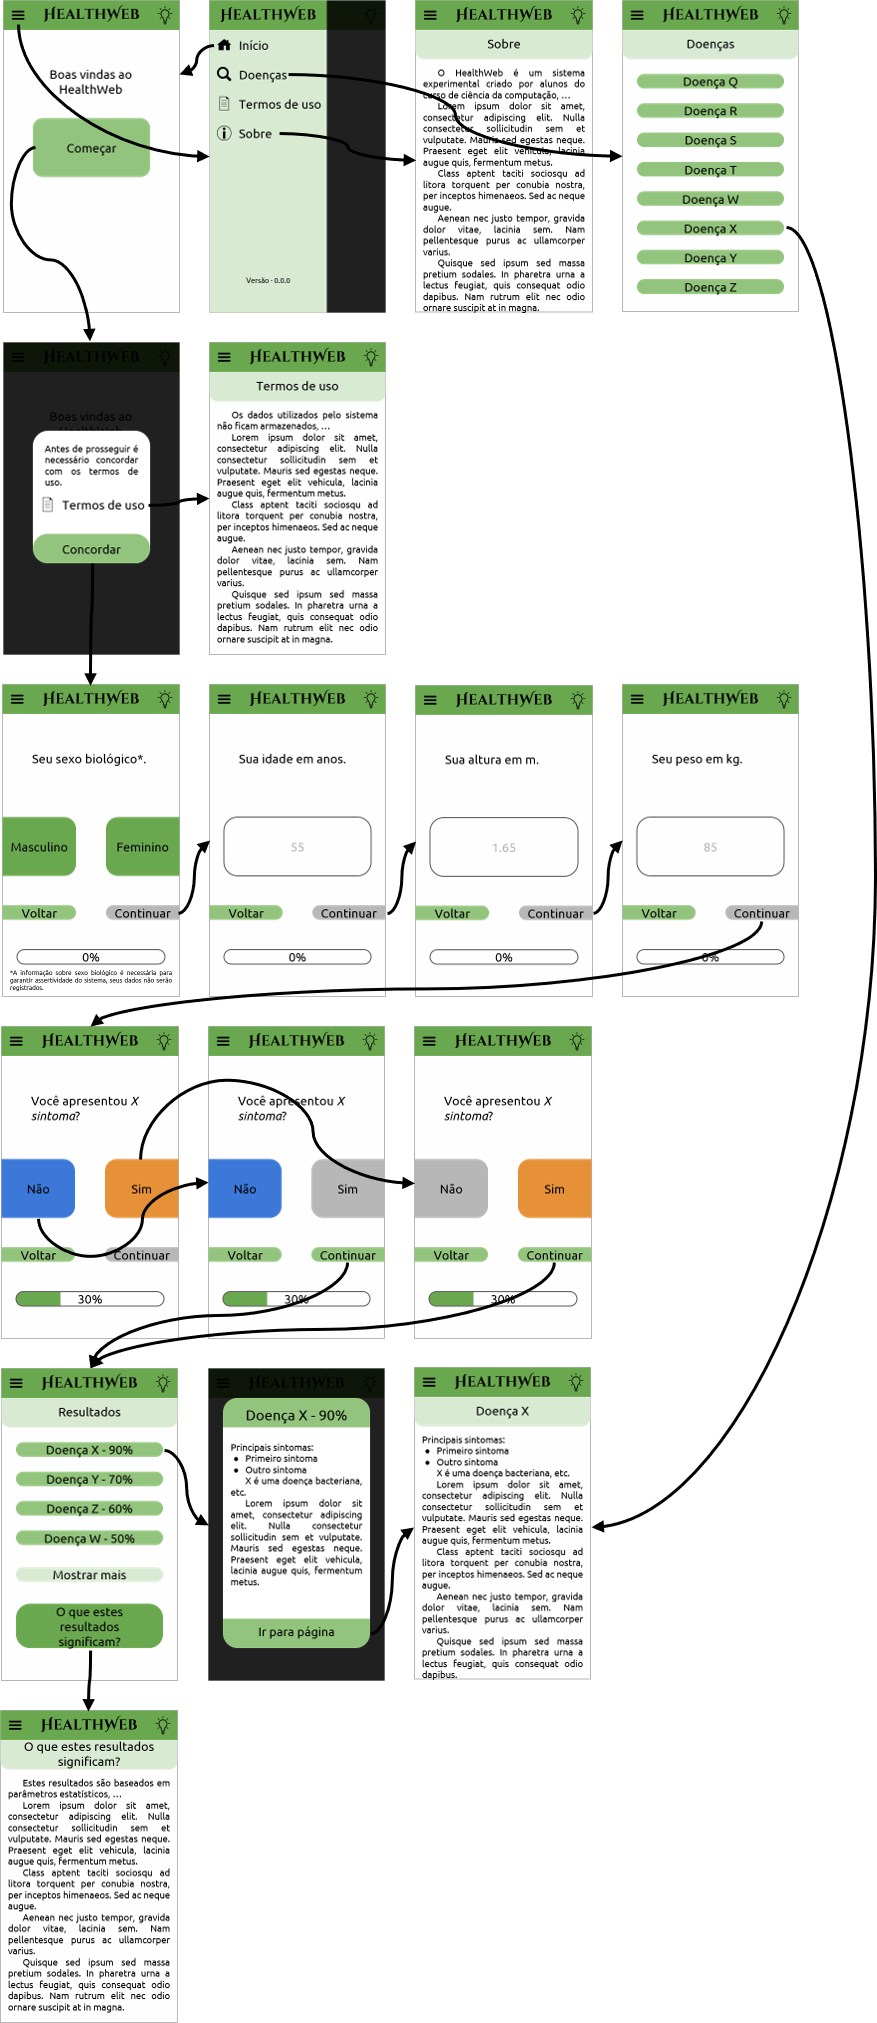
\includegraphics[height=\textheight]{figure/prototype/mobile/storyboard.png}
	\caption{Storyboard para versão mobile.}
	\label{fig:logomarca}
\end{figure}

\subsection{Versão desktop}

\begin{figure}[h]
	\centering
	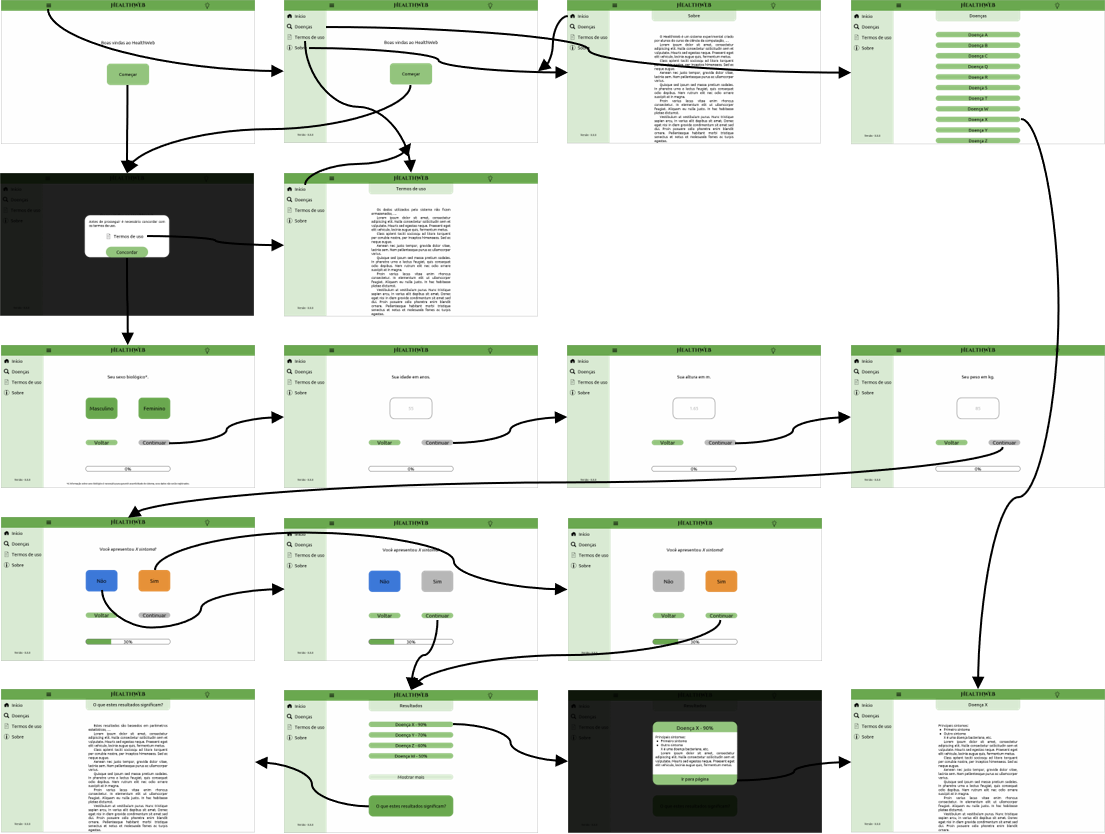
\includegraphics[width=\linewidth]{figure/prototype/desktop/storyboard.png}
	\caption{Storyboard para versão desktop.}
	\label{fig:logomarca}
\end{figure}